%%%%%%%%%%%%%%%%%%%%%%%%%%%%%%%%%%%%%%%%%%%%%%%%%%%%%%%%%%%%%%%%%%%%%%%%%%%%%%%%%%%%
%Do not alter this block of commands.  If you're proficient at LaTeX, you may include additional packages, create macros, etc. immediately below this block of commands, but make sure to NOT alter the header, margin, and comment settings here. 
\documentclass[12pt]{article}
 \usepackage[margin=1in]{geometry}
 \usepackage{tikz, tikz-3dplot}
 \usepackage{caption}
\usepackage{amsmath,amsthm,amssymb,amsfonts, enumitem, fancyhdr, color, comment, graphicx, environ}
\pagestyle{fancy}
\setlength{\headheight}{65pt}
\newenvironment{problem}[2][Problem]{\begin{trivlist}
\item[\hskip \labelsep {\bfseries #1}\hskip \labelsep {\bfseries #2.}]}{\end{trivlist}}
\newenvironment{sol}
{\emph{Solution:}
}
{
    \qed
    }
\specialcomment{com}{ \color{blue} \textbf{Comment:} }{\color{black}} %for instructor comments while grading
\NewEnviron{probscore}{\marginpar{ \color{blue} \tiny Problem Score: \BODY \color{black} }}
%%%%%%%%%%%%%%%%%%%%%%%%%%%%%%%%%%%%%%%%%%%%%%%%%%%%%%%%%%%%%%%%%%%%%%%%%%%%%%%%%





%%%%%%%%%%%%%%%%%%%%%%%%%%%%%%%%%%%%%%%%%%%%%
%Fill in the appropriate information below
\lhead{Hyukdong Kim}  %replace with your name
\rhead{Elementary Math \\ Computational PDE \\ Semester 1 \\ Assignment 3} %replace XYZ with the homework course number, semester (e.g. ``Spring 2019"), and assignment number.
%%%%%%%%%%%%%%%%%%%%%%%%%%%%%%%%%%%%%%%%%%%%%


%%%%%%%%%%%%%%%%%%%%%%%%%%%%%%%%%%%%%%
%Do not alter this block.
\begin{document}
%%%%%%%%%%%%%%%%%%%%%%%%%%%%%%%%%%%%%%


%Solutions to problems go below.  Please follow the guidelines from https://www.overleaf.com/read/sfbcjxcgsnsk/


%Copy the following block of text for each problem in the assignment.
Find the torsion of the followings.
\begin{problem}{1} 
    $r=r(t)=(a \cos t, a \sin t, bt)$ s.t. $a>0, b \neq 0, t \in \mathbb{R}$.
\end{problem}

\begin{sol}

\begin{align*}
    r(t)  &= (a \cos{t}, a \sin{t}, bt) \\
    r'(t) &= (-a \sin{t}, a \cos{t}, b)
\end{align*}
\begin{align}
    s(t) = \int_0^t \left\lVert r'(t) \right\rVert_2 dx 
        &= \int_0^t \sqrt{(-a \sin{t})^2 + (a \cos{t})^2+b ^2} dx \nonumber \\
        &= \int_0^t \sqrt{a^2 \sin^2{t} + a^2 \cos^2{t} + b^2} dx = \sqrt{a^2+b^2}t \label{eq:s} 
\end{align}
From equation \ref{eq:s}, let $t=\frac{s}{\sqrt{a^2+b^2}}$.
\begin{align}
    \tilde{r}(t)   &= \tilde{r} \left(\frac{s}{\sqrt{a^2+b^2}} \right) 
                        = \left(a \cos{\frac{s}{\sqrt{a^2+b^2}}}, 
                                a \sin{\frac{s}{\sqrt{a^2+b^2}}}, 
                                b \frac{s}{\sqrt{a^2+b^2}}\right) \nonumber\\
    \tilde{r}'(t)  &= \left(-\frac{a}{\sqrt{a^2+b^2}} \sin{\frac{s}{\sqrt{a^2+b^2}}}, 
                             \frac{a}{\sqrt{a^2+b^2}} \cos{\frac{s}{\sqrt{a^2+b^2}}}, 
                            \frac{b}{\sqrt{a^2+b^2}} \right) \nonumber\\
    \tilde{r}''(t) &= \left(-\frac{a}{a^2+b^2} \cos{\frac{s}{\sqrt{a^2+b^2}}}, 
                            -\frac{a}{a^2+b^2} \sin{\frac{s}{\sqrt{a^2+b^2}}}, 
                            0 \right) \label{eq:r''}
\end{align}
From equation \ref{eq:r''}, curvature $\kappa$ is
\begin{align}
    \kappa(s) = \left\lVert \tilde{r}''(t) \right\rVert_2 
        &= \sqrt{
            \left( -\frac{a}{a^2+b^2} \cos{\frac{s}{\sqrt{a^2+b^2}}} \right)^2
            + \left( -\frac{a}{a^2+b^2} \sin{\frac{s}{\sqrt{a^2+b^2}}} \right)^2
            + 0^2
            } \nonumber \\
        &= \sqrt{
            \left( -\frac{a}{a^2+b^2} \right)^2 
            \left( \cos^2{\frac{s}{\sqrt{a^2+b^2}}} + \sin^2{\frac{s}{\sqrt{a^2+b^2}}} \right)}
             = \frac{a}{a^2+b^2} \nonumber
\end{align}
On the other hand, from $n(s) := \frac{1}{\kappa (s)} \tilde{r}''(t)$,
\begin{align}
    n(s) &= \frac{1}{\kappa (s)} \tilde{r}''(t) \nonumber\\
         &= \frac{a^2+b^2}{a} \cdot \left(-\frac{a}{a^2+b^2} \cos{\frac{s}{\sqrt{a^2+b^2}}}, -\frac{a}{a^2+b^2} \sin{\frac{s}{\sqrt{a^2+b^2}}}, 0 \right) \nonumber\\
         &= \left(-\cos{\frac{s}{\sqrt{a^2+b^2}}}, -\sin{\frac{s}{\sqrt{a^2+b^2}}}, 0 \right) \nonumber
\end{align}
On the other hand, from $b'(s) = t(s) \times n'(s)$,
\begin{align}
    b'(s)=\tilde{r}'(t) \times n'(s)
    &= 
    \begin{bmatrix} 
        \tilde{r}'(t)_2 \cdot n'(s)_3 - \tilde{r}'(t)_3 \cdot n'(s)_2 \\
        \tilde{r}'(t)_3 \cdot n'(s)_1 - \tilde{r}'(t)_1 \cdot n'(s)_3 \\
        \tilde{r}'(t)_1 \cdot n'(s)_2 - \tilde{r}'(t)_2 \cdot n'(s)_1 
    \end{bmatrix} \nonumber \\
    &= 
    \begin{bmatrix}
        \frac{a}{\sqrt{a^2+b^2}} \cos{\frac{s}{\sqrt{a^2+b^2}}}                \cdot 0                                             \\
        \frac{b}{\sqrt{a^2+b^2}}                                               \cdot \left( \frac{1}{\sqrt{a^2+b^2}} \sin{\frac{s}{\sqrt{a^2+b^2}}}\right)  \\
        \left(-\frac{a}{\sqrt{a^2+b^2}} \sin{\frac{s}{\sqrt{a^2+b^2}}} \right) \cdot \left(-\frac{1}{\sqrt{a^2+b^2}} \cos{\frac{s}{\sqrt{a^2+b^2}}}\right)  
    \end{bmatrix} \nonumber \\
    &\qquad-
    \begin{bmatrix}
        \frac{b}{\sqrt{a^2+b^2}}                                               \cdot \left(-\frac{1}{\sqrt{a^2+b^2}} \cos{\frac{s}{\sqrt{a^2+b^2}}}\right) \\
        \left(-\frac{a}{\sqrt{a^2+b^2}} \sin{\frac{s}{\sqrt{a^2+b^2}}} \right) \cdot 0                                            \\
        \frac{a}{\sqrt{a^2+b^2}} \cos{\frac{s}{\sqrt{a^2+b^2}}}                \cdot \left( \frac{1}{\sqrt{a^2+b^2}} \sin{\frac{s}{\sqrt{a^2+b^2}}}\right)
    \end{bmatrix} \nonumber \\
    &=
    \begin{bmatrix}
        \frac{b}{a^2+b^2} \cos{\frac{s}{\sqrt{a^2+b^2}}} \\
        \frac{b}{a^2+b^2} \sin{\frac{s}{\sqrt{a^2+b^2}}} \\
        0 \nonumber
    \end{bmatrix}
\end{align}
From $b'(s)=\tau(s)(-n(s))$,
\begin{align}
    b'(s)&=\tau(s)(-n(s)) \nonumber \\
    \Leftrightarrow \tau(s)&=-b'(s) \cdot n(s) \nonumber \\
    &=-\left[ \frac{b}{a^2+b^2} \cos{\frac{s}{\sqrt{a^2+b^2}}}, \frac{b}{a^2+b^2} \sin{\frac{s}{\sqrt{a^2+b^2}}}, 0 \right] \nonumber
    \begin{bmatrix}
        -\cos{\frac{s}{\sqrt{a^2+b^2}}} \\
        -\sin{\frac{s}{\sqrt{a^2+b^2}}} \\
        0
    \end{bmatrix}\\
    &= \frac{b}{a^2+b^2} \cos^2{\frac{s}{\sqrt{a^2+b^2}}} + \frac{b}{a^2+b^2} \sin^2{\frac{s}{\sqrt{a^2+b^2}}} + 0 \nonumber \\
    &= \frac{b}{a^2+b^2} \left( \cos^2{\frac{s}{\sqrt{a^2+b^2}}}+\sin^2{\frac{s}{\sqrt{a^2+b^2}}} \right) = \frac{b}{a^2+b^2} \nonumber
\end{align}
$$\therefore \tau(s)=\frac{b}{a^2+b^2}$$
\end{sol}

\begin{minipage}[t]{0.45\linewidth}
    \centering
    \begin{tikzpicture}[scale=1.5]
        \pgfmathsetmacro{\a}{1} % set a
        \pgfmathsetmacro{\b}{0.5} % set b
        \draw[->] (0,0,0) -- (2,0,0) node[right]{$y$};
        \draw[->] (0,-1.5,0) -- (0,1.5,0) node[above]{$z$};
        \draw[->] (0,0,0) -- (0,0,2) node[below left]{$x$};
        \draw[blue,thick,domain=0:5.5 *pi,samples=200,smooth] plot ({\a*sin(deg(\x))},{\b*\x/(2*pi)},{\a*cos(deg(\x))});
    \end{tikzpicture}
    \captionof{figure}{Helix with $b > 0$}
  \end{minipage}%
  \begin{minipage}[t]{0.5\linewidth}
    \centering
    \begin{tikzpicture}[scale=1.5]
        \pgfmathsetmacro{\a}{1} % set a
        \pgfmathsetmacro{\b}{-0.5} % set b
        \draw[->] (0,0,0) -- (2,0,0) node[right]{$y$};
        \draw[->] (0,-1.5,0) -- (0,1.5,0) node[above]{$z$};
        \draw[->] (0,0,0) -- (0,0,2) node[below left]{$x$};
        \draw[blue,thick,domain=0:5.5*pi,samples=200,smooth] plot ({\a*sin(deg(\x))},{\b*\x/(2*pi)},{\a*cos(deg(\x))});
    \end{tikzpicture}
    \captionof{figure}{Helix with $b < 0$}
\end{minipage}

%Copy the following block of text for each problem in the assignment.
% \begin{problem}{x.y.z}
% Statement of problem goes here (write the problem exactly as it appears in the book).
% \end{problem}
% \begin{sol}
% Write your solution here.
% \end{sol}





%%%%%%%%%%%%%%%%%%%%%%%%%%%%%%%%%%%%%
%Do not alter anything below this line.
\end{document}